\section{Datenvorverarbeitung}
Zu Beginn der Vorverarbeitung ist es zunächst notwendig den Informationsgehalt des Open Source Datensatzes zu analysieren. Im Anschluss daran können in der Datenaufbereitung fehlende Werte interpoliert und Ausreißer gefiltert werden.

\subsection{Beschreibung des Datensatzes}
Der in dieser Arbeit verwendete Datensatz wurde von \textsc{Thabtah} \cite{Thabtah2017, Thabtah}, im Zuge seiner Arbeit zur Erstellung eines Konzepts für die Diagnose einer ASS, im Umfang von 704 Testresultaten gesammelt und veröffentlicht. Die Datensammlung basiert dabei auf den von der Organisation \textsc{NICE} \cite{NICE2012} beschriebenen Richtlinien zur Diagnose einer ASS mit Hilfe des AQ\footnote{\label{foot:3}Test zur Berechnung des Autismus-Spektrum-Quotienten.}-10. Eine Beschreibung des Datensatzes liegt der Veröffentlichung bei, enthält jedoch fehlerhafte sowie unzureichende Informationen und Zuordnungen. Hierzu wird im Rahmen dieser Arbeit der veröffentlichte Datensatz ergänzt und in Tabelle \ref{tbl:datensatz} beschrieben.

\begin{table}[htbp]
\caption{Der Aufbau des Open Source Datensatzes}
\begin{tabular}{l p{6cm}}
\textbf{Attribut-Name} & \textbf{Beschreibung}\\ \hline
age & Alter in Jahren\\
gender & Geschlecht männlich / weiblich\\
ethnicity & Ethnische Herkunft der Person\\
jaundice	 & Mit Gelbsucht geboren\\
autism & Autismus-Diagnose innerhalb der Familie\\
relation & Person, die das Testverfahren durchführt\\
country of residence & Land des Wohnsitzes  \\
used app before & Screening-App bereits zuvor benutzt\\
age desc & Gruppierung des Testverfahrens anhand des Alters\\
A1 & Antwort zur Frage 1 (Trifft zu = 1, sonst = 0)\\
A2 & Antwort zur Frage 2 (Trifft zu = 0, sonst = 1)\\
A3 & Antwort zur Frage 3 (Trifft zu = 0, sonst = 1)\\
A4 & Antwort zur Frage 4 (Trifft zu = 0, sonst = 1)\\
A5 & Antwort zur Frage 5 (Trifft zu = 1, sonst = 0)\\
A6 & Antwort zur Frage 6 (Trifft zu = 0, sonst = 1)\\
A7 & Antwort zur Frage 7 (Trifft zu = 1, sonst = 0)\\
A8 & Antwort zur Frage 8 (Trifft zu = 0, sonst = 1)\\
A9 & Antwort zur Frage 9 (Trifft zu = 0, sonst = 1)\\
A10 & Antwort zur Frage 10 (Trifft zu = 1, sonst = 0)\\
result & Anhand der Antworten errechnetes Gesamtresultat\\
classifiedASD & Mögliche diagnostizierte ASS\\
\end{tabular}
\centering
\label{tbl:datensatz}
\end{table}

\subsection{Datenanalyse und -aufbereitung} \label{sec:analysis}
Das Verfahren zur Zuordnung der einzelnen Datensätze zu den Werten in \textit{classifiedASD} wurde nach \textsc{Thabtah} \cite{Thabtah2017} dabei anhand der von \textsc{NICE} \cite{NICE2012} beschriebenen Richtlinien zur ASS-Diagnose durchgeführt. Dies führt zur in Abbildung \ref{fig:result_classification} dargestellten Verteilung der Daten anhand der Spalten \textit{result} und \textit{classifiedASD}. Dabei ist erkennbar, dass eine eindeutige Zuordnung bereits mit Hilfe der Spalte \textit{result} durchführbar ist.

\begin{figure}[h!]
\centering
% This file was created by matplotlib2tikz v0.6.17.
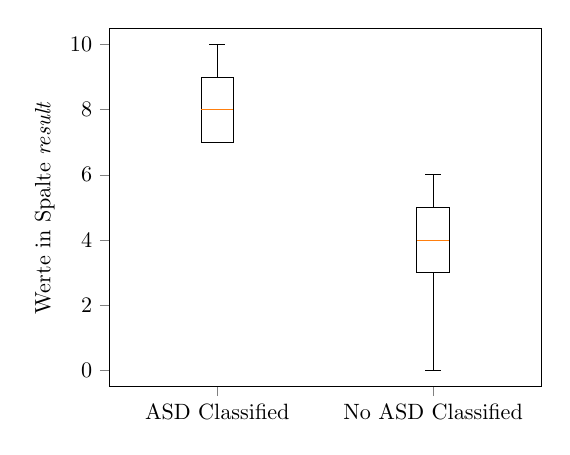
\begin{tikzpicture}[scale=.8,transform shape]

\definecolor{color0}{rgb}{1,0.498039215686275,0.0549019607843137}

\begin{axis}[
ylabel={Werte in Spalte \textit{result}},
xmin=0.5, xmax=2.5,
ymin=-0.5, ymax=10.5,
xtick={1,2},
xticklabels={ASD Classified,No ASD Classified},
tick align=outside,
tick pos=left,
x grid style={white!69.01960784313725!black},
y grid style={white!69.01960784313725!black}
]
\addplot [black, forget plot]
table {%
0.925 7
1.075 7
1.075 9
0.925 9
0.925 7
};
\addplot [black, forget plot]
table {%
1 7
1 7
};
\addplot [black, forget plot]
table {%
1 9
1 10
};
\addplot [black, forget plot]
table {%
0.9625 7
1.0375 7
};
\addplot [black, forget plot]
table {%
0.9625 10
1.0375 10
};
\addplot [black, forget plot]
table {%
1.925 3
2.075 3
2.075 5
1.925 5
1.925 3
};
\addplot [black, forget plot]
table {%
2 3
2 0
};
\addplot [black, forget plot]
table {%
2 5
2 6
};
\addplot [black, forget plot]
table {%
1.9625 0
2.0375 0
};
\addplot [black, forget plot]
table {%
1.9625 6
2.0375 6
};
\addplot [color0, forget plot]
table {%
0.925 8
1.075 8
};
\addplot [color0, forget plot]
table {%
1.925 4
2.075 4
};
\end{axis}

\end{tikzpicture}
\caption{\em Zuordnung der Datensätze in Abhängigkeit der Werte des Attributes \glqq \textit{result}\grqq}
\label{fig:result_classification}
\end{figure}

Im Verlauf der Arbeit werden jedoch auch weitere Merkmale verwendet, um die Klassifikation anhand der abgegebenen Antworten und Verhaltensweisen der Personen zu untersuchen. Um weitere Merkmale verwenden zu können, wird hierzu eine Datenaufbereitung durchgeführt.

% Vorverarbeitung 
%		-> Fehler ausgebessert / gefiltert
%		-> Normalisierung
%		-> usw..
%		-> Reduktion macht hierbei keinen Sinn! Daten sind bereits stark vereinfacht
Innerhalb der Datenaufbereitung werden in der ersten Analyse Ausreißer mit fehlerhaften und fehlenden Informationen herausgefiltert. Dabei werden aufgrund von fehlenden Informationen bei den Attributen \textit{ethnicity}, \textit{relation} und \textit{age}, 95 Datensätze für die weitere Verarbeitung entfernt.

Für eine eindeutige Klassifikation ist es außerdem notwendig, die in den Attributen \textit{jaundice} und \textit{autism} enthaltenen nominalen Werte entsprechend zu normalisieren. Hierbei werden die bool'schen Werte \glqq yes\grqq{} und \glqq no\grqq{} zu den numerischen Werten $1$ für \glqq yes\grqq{} und $0$ für \glqq no\grqq{} abgeändert. 

Die ordinalen Werte im Attribut \textit{relation} werden mit Hilfe der \glqq 1-aus-n\grqq{} (engl. \glqq one-hot\grqq) Kodierung aufbereitet. Dies bedeutet, dass für jeden Wert des Attributes eine neue Spalte erzeugt wird. Dabei wird der Wert in der zugehörigen Spalte auf $1$ und in allen anderen Spalten des Attributes auf $0$ gesetzt. %Dies ergibt eine Matrix in der einer Person (repräsentiert durch eine Zeile $i$) ein einziger Wert des Attributes durch eine Markierung der Spalte $j$ mit Hilfe der Funktion $f_{\text{relation}}(i,j)=1$ zugewiesen wird.

Abschließend werden die numerischen Werte $x$ eines Attributes $X$ normiert. In der Normierung der Attribute \textit{age} und \textit{result} wird dabei der maximale Wert des Attributes errechnet und der Anteil des aktuellen Wertes an dem maximalen Wert als normierter Wert ermittelt ($f_{\text{Normierung}}(x) = \frac{x}{\max(X)}$). Somit ergibt sich eine Normierung der Werte im Intervall $[0,1]$.

